\section{Struttura del progetto}
Tutto il progetto è strutturato in 4 \emph{package(Dataset,RFD,Actors,Utility)}.
Nel corso della descrizione del codice, assumeremo che il lettore possieda già basi del linguaggio di programmazione \emph{Java}. Per cui, sarà omessa la differenziazione tra metodi pubblici, metodi privati e metodi statici delle singole classi.
Sia la \textbf{matrice delle distanze}, sia il \textbf{dataset} sono implementati utilizzando due diversi data frame (classe \texttt{DataFrame} della libreria DataFrame di Joinery citata nella sezione precedente). Per gli \textbf{insiemi C}, invece, è stata utilizzata una lista (classe \texttt{ObjectArrayList} della libreria FastUtil) avente come elementi i vettori contenenti le distanze e  le coppie di identificativi delle due tuple da cui tale vettore è stato ricavato.
Le \textbf{RFDs} sono state inserite in una classe di utility chiamata \textbf{RFDMap}.
\begin{figure}[H]
	\centering
	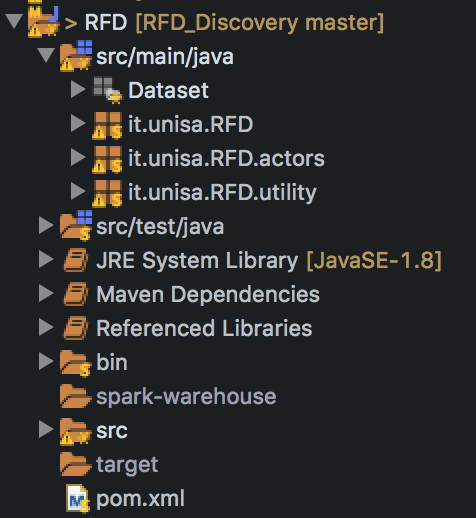
\includegraphics{Immagini/StrutturaProgetto.png}
	\caption{Struttura del Progetto}
	\label{fig:StrutturaProgetto}
\end{figure}
\subsection{Package DataSet}
Il package DataSet include una serie di DataSet in formato $csv$. I DataSet inclusi nel progetto sono:
\begin{itemize}[noitemsep]
	\let\labelitemi\labelitemii
	\item adult.csv
	\item balance-scale.csv
	\item breast-cancer-wisconsin.csv
	\item bridges.csv
	\item chess.csv
	\item Citiseer.csv
	\item cora.csv
	\item crawled-tweets.csv
	\item dataset.csv
	\item dataset{\_}string.csv
	\item echocardiogram.csv
	\item hepatitis.csv
	\item horse.csv
	\item iris.csv
	\item restaurant.csv
\end{itemize}
\subsection{Package RFD}
Questo pacchetto contiene le classi che vengono utilizzate per le fasi principali del nostro algoritmo.\\
\begin{figure}[H]
	\centering
	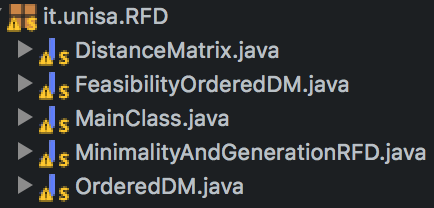
\includegraphics{Immagini/PackageRFD.png}
	\caption{Package RFD}
	\label{fig:Package RFD}
\end{figure}
Il contenuto di questo pacchetto è:\\
\textbf{DistanceMatrix.java}:
Questa classe contiene alcuni metodi statici fondamentali per il caricamento del dataset nella struttura dati \emph{DataFrame} e per la creazione della Distance Matrix,tali metodi verranno spiegati di seguito.
\begin{listing}[H]
	\inputminted[]{java}{Codici/loadDF.java}
	\caption{Metodo loadDF}
	\label{Code:1}
\end{listing}
Il metodo \textbf{loadDF} è utilizzato per importare il dataset dato in input come file csv.
Per importare tale file ci siamo affidati al metodo messo a disposizione dalla libreria DataFrame di Joinery.Tale metodo ha il compito di caricare il file CSV e di trasformarlo in un oggetto della classe \texttt{DataFrame} di Joinery. Tutti i parametri relativi al CSV specificati nella firma saranno usati per interpretare correttamente tale file. Restituisce un oggetto di tipo \texttt{DataFrame} contenente il dataset. \\
Gli argomenti da passare al metodo sono i seguenti:
\begin{itemize}
	\item \textbf{nameCSV} : il percorso dal quale caricare il file CSV;
	\item \textbf{separator}:  il separatore di campi del file CSV;
	\item \textbf{naString}: il carattere di valore nullo presente all'interno del file CSV;
	\item \textbf{hasHeader}: presenza o meno dell'header come prima riga nel file CSV;
	\item \textbf{righeTaglio}: permette di effettuare un taglio sulle righe, inserire "0" se non si vuole effettuare alcun taglio.
	Tale parametro è stato inserito al fine di effettuare testing sulle grandezze dei dataset.
\end{itemize}
Durante l'esecuzione del nostro algoritmo è necessario calcolare un secondo dataset che nel nostro caso andrà ad essere inserito in una istanza della classe DataFrame di joinery.
Questo secondo dataset è la matrice delle distanze che conterrà, per ogni coppia di pattern nel dataset originale, la differenza dei valori dei singoli attributi.
Per calcolare la differenza fra i valori di un attributo, occorre prima di tutto capire il tipo dell'attributo in questione. Per questo scopo viene utilizzato il metodo offerto dalla classe DataFrame di Joinery: \textbf{types()}.
A differenza del dataset originale, la matrice delle distanze avrà un campo in più inserito alla fine che rappresenterà la coppia dei pattern da cui è nata quella riga.
Tale processo di creazione farà in modo di inserire una sola riga tra una coppia di tipo (1,2) e (2,1).
Infine, effettuiamo un taglio delle righe duplicate.
Tutto questo viene effettuato dal metodo \textbf{concurrentCreateMatrix}.
\begin{listing}[H]
	\inputminted[]{java}{Codici/CreateDistanceMatrix.java}
	\caption{Metodo CreateDistanceMatrix}
	\label{Code:2}
\end{listing}
Gli argomenti da passare al metodo sono i seguenti:
\begin{itemize}
	\item \textbf{inizio} : indice di riga di inizio del processo di creazione della matrice delle distanze su cui il thread corrente dovrà operare;
	\item \textbf{dimensione}: numero di righe su cui operare per il thread corrente;
	\item \textbf{completeDF}: dataframe precedentemente importato.
\end{itemize}
Come ultimo metodo richiamato dalla classe \textbf{DistanceMatrix} c'è \textbf{createOrderedDM}, questo metodo viene utilizzato per creare informazioni sulla matrice delle distanze al variare di tutti gli \emph{RHS}.
Queste informazioni saranno memorizzate come istanza di una classe di utility chiamata \textbf{OrderedDM}
\begin{listing}[H]
	\inputminted[]{java}{Codici/OrderedDMMethod.java}
	\caption{Metodo OrderedDMMethod}
	\label{Code:3}
\end{listing}
Gli argomenti da passare al metodo sono i seguenti:
\begin{itemize}
	\item \textbf{indiceRHS} : indice di colonna del corrente RHS;
	\item \textbf{dm}: matrice delle distanze creata in precedenza .
\end{itemize}
\textbf{FeasibilityOrderedDM.java}:
Questa classe contiene i metodi per l'esecuzione della fase di \emph{Feasibility}, che ricordiamo essere la prima fase dell'algoritmo di RFD Discovery.\\
Il metodo più importante di questa classe è senz'altro il metodo statico \textbf{feasibilityTest}, esso darà inizio alla fase vera e propria di Feasibility.
Questo metodo restituirà gli insiemi C fondamentali per l'inizio della prossima fase di \emph{Minimality}.
\begin{listing}[H]
	\inputminted[]{java}{Codici/FeasibilityTest.java}
	\caption{Metodo FeasibilityTest}
	\label{Code:4}
\end{listing}
Gli argomenti da passare al metodo sono i seguenti:
\begin{itemize}
	\item \textbf{orderedDM} : istanza di una classe di utility che contiene informazioni sulla matrice delle distanze per un dato RHS;
	\item \textbf{dmGenerale}: matrice delle distanze creata in precedenza .
\end{itemize}
Questo metodo richiamerà, come visto nel capitolo precedente la dominanza tra due righe.
La dominanza è definita attraverso un altro metodo implementato in questa classe.
Il metodo è chiamato \textbf{dominance} e restituisce true se la prima tupla passata come parametro \emph{domina} la seconda.
\begin{listing}[H]
	\inputminted[]{java}{Codici/Dominance.java}
	\caption{Metodo Dominance}
	\label{Code:5}
\end{listing}
Gli argomenti da passare al metodo sono i seguenti:
\begin{itemize}
	\item \textbf{tupla1} : una riga per il confronto;
	\item \textbf{tupla2} : seconda riga per il confronto;
	\item \textbf{dmGenerale}: matrice delle distanze creata in precedenza .
	\item \textbf{rhs} : indice di colonna che rappresenta l'RHS attualmente considerato;
\end{itemize}
\textbf{MinimalityAndGenerationRFD.java}:
Questa classe contiene il metodo per l'inizio delle ultime due fasi finali.
Durante l'esecuzione si cercano i minimi attraverso la fase di \emph{Minimality} e, successivamente, vengono trovate le \emph{RFD} durante la fase di \emph{RFD Generation}(Queste ultime due fasi non sono parte dello studio di questo lavoro di tesi).
Il Metodo che si occupa di dare inizio a questi ultimi due step è \textbf{startMinimalityAndGeneration}.
\begin{listing}[H]
	\inputminted[]{java}{Codici/MinimalityAndGenerationRFD.java}
	\caption{Metodo MinimalityAndGenerationRFD}
	\label{Code:6}
\end{listing}
Gli argomenti da passare al metodo sono i seguenti:
\begin{itemize}
	\item \textbf{allC} : insiemi C trovati nella fase precedente di Feasibility;
	\item \textbf{colonne} : numero colonne del dataset;
	\item \textbf{orderedDM}:  istanza di una classe di utility che contiene informazioni sulla matrice delle distanze per un dato RHS;
	\item \textbf{dM} : matrice delle distanze.
\end{itemize}
\textbf{MainClass.java}:
Classe che da il via al nostro algoritmo, si occupa di creare il container per i nostri attori(\emph{ActorSystem}) e di mandare un messaggio all'\emph{Actor principale} per l'avvio delle varie fasi dell'algoritmo.
Di seguito vediamo uno snippet che mostra quanto appena descritto.
\begin{listing}[H]
	\inputminted[]{java}{Codici/MainClass.java}
	\caption{MainClass}
	\label{Code:7}
\end{listing}
\textbf{OrderedDM.java}:
Classe di utility per mantenere in memoria informazioni sulla matrice delle distanze per i vari RHS.\\
Le variabili di istanza di tale classe sono le seguenti:
\begin{itemize}
	\item \textbf{allC} : insiemi C trovati nella fase precedente di Feasibility;
	\item \textbf{rhs} : indice di colonna che rappresenta l'RHS attualmente considerato;
	\item \textbf{lhs} : lista degli indici colonna degli LHS.
\end{itemize}
\subsection{Package Actors}
\begin{figure}[H]
	\centering
	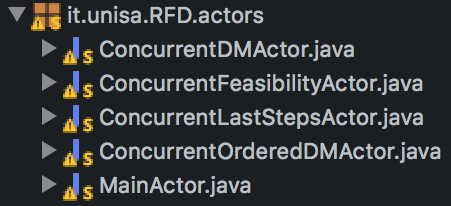
\includegraphics{Immagini/PackageActors.png}
	\caption{Package Actors}
	\label{fig:Package Actors}
\end{figure}
Questo pacchetto contiene le classi che rappresentano gli \emph{Actors}.
Queste classi si occupano di richiamare i metodi presenti nel package RFD in modo concorrente.
Verrà istanziato un attore presente in questo pacchetto per quanti thread vogliamo far lavorare in concorrenza per ogni fase dell'algoritmo.
Le classi per questo pacchetto sono:\\
\textbf{MainActor.java}:
Classe principale che coordina il numero di attori che devono essere istanziati.
Questa classe da il via ad ogni singola fase dell'algoritmo richiamando i metodi principali situati nelle classi del pacchetto precedentemente visto(RFD).
Per ogni inizio di fase istanzia un numero di attori(thread) deciso come parametro da parte dell'utente(default:2).\\
Di seguito è riportato un esempio di lancio di messaggio da parte del \emph{MainActor}, in particolare, in questo esempio viene lanciato un thread per la creazione di una parte di matrice delle distanze.\\
\begin{listing}[H]
	\inputminted[]{java}{Codici/CreateMatrixMessage.java}
	\caption{Esempio invio messaggio da MainActor}
	\label{Code:8}
\end{listing}
\textbf{ConcurrentDMActor.java}:
Questa classe, istanziata in numero pari ai thread desiderati in input, è la responsabile della creazione della matrice delle distanze. Essa riceve un messaggio da parte del \emph{MainActor} e richiama il metodo \textbf{concurrenceCreateMatrix}.
A lavoro ultimato invierà la sua parte di matrice delle distanze appena calcolata al MainActor. Il MainActor, infine, ricompone tutte le parti ricevute dai diversi thread ed elimina eventuali pattern ripetuti. Al termine otterremo la matrice delle distanze completa che verrà utilizzata nelle fasi successive.
\begin{listing}[H]
	\inputminted[]{java}{Codici/ConcurrentDMActor.java}
	\caption{Chiamata metodo concurrentCreateMatrix}
	\label{Code:9}
\end{listing}
\textbf{ConcurrentOrderedDMActor.java}:
Questa classe attende un messaggio da parte del \emph{MainActor} per dare il via alla fase di creazione degli \emph{OrderedDM} richiamando l'apposito metodo nella classe DistanceMatrix.\\
\begin{listing}[H]
	\inputminted[]{java}{Codici/ConcurrentOrderedDMActor.java}
	\caption{Chiamata metodo createOrderedDM}
	\label{Code:10}
\end{listing}
\textbf{ConcurrentFeasibilityActor.java}:
Analogamente alle classi precedenti di attori, essa viene istanziata in numero pari ai thread desiderati.
Queste istanze attendono un messaggio per dare il via alla fase di \emph{Feasibility} chiamando il metodo della classe \emph{FeasibilityOrderedDM}.\\
\begin{listing}[H]
	\inputminted[]{java}{Codici/ConcurrentFeasibilityActor.java}
	\caption{Chiamata metodo feasibilityTest}
	\label{Code:11}
\end{listing}
\textbf{ConcurrentLastStepsActor.java}:
Questa classe attende un messaggio da parte del \emph{MainActor} per dare il via alle ultime due fasi di \emph{Minimality} e \emph{RFD Generation}.
Le due fasi hanno inizio chiamando il metodo apposito nella classe \emph{MinimalityAndGenerationRFD}.
\begin{listing}[H]
	\inputminted[]{java}{Codici/ConcurrentLastStepsActor.java}
	\caption{Chiamata metodo startMinimalityAndGeneration}
	\label{Code:12}
\end{listing}
\subsection{Package Utility}
\begin{figure}[H]
	\centering
	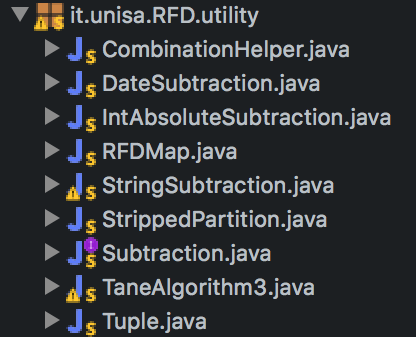
\includegraphics{Immagini/PackageUtility.png}
	\caption{Package Utility}
	\label{fig:Package Utility}
\end{figure}
Questo pacchetto contiene le classi di utility utilizzate durante i 3 processi dell'algoritmo.
Tale package comprende l'interfaccia per i vari tipi di differenza tra i campi e le relative implementazioni.
In particolare, possiamo notare la presenza di 3 diversi tipi di differenze: \emph{Interi},\emph{Date},\emph{String}. Particolare attenzione può essere posta sulla differenza tra stringhe. Quest'ultima è effettuata tramite l'algoritmo di \emph{levenshtein}.